%%
%% This is file `sample-authordraft.tex',
%% generated with the docstrip utility.
%%
%% The original source files were:
%%
%% samples.dtx  (with options: `authordraft')
%% 
%% IMPORTANT NOTICE:
%% 
%% For the copyright see the source file.
%% 
%% Any modified versions of this file must be renamed
%% with new filenames distinct from sample-authordraft.tex.
%% 
%% For distribution of the original source see the terms
%% for copying and modification in the file samples.dtx.
%% 
%% This generated file may be distributed as long as the
%% original source files, as listed above, are part of the
%% same distribution. (The sources need not necessarily be
%% in the same archive or directory.)
%%
%% Commands for TeXCount
%TC:macro \cite [option:text,text]
%TC:macro \citep [option:text,text]
%TC:macro \citet [option:text,text]
%TC:envir table 0 1
%TC:envir table* 0 1
%TC:envir tabular [ignore] word
%TC:envir displaymath 0 word
%TC:envir math 0 word
%TC:envir comment 0 0
%%
%%
%% The first command in your LaTeX source must be the \documentclass command.
 \documentclass[sigconf, 10pt]{acmart}
%% NOTE that a single column version may required for 
%% submission and peer review. This can be done by changing
%% the \doucmentclass[...]{acmart} in this template to 
%% \documentclass[manuscript,screen]{acmart}
%% 
\usepackage{algorithm}
\usepackage{amsmath}
\usepackage{algorithmic}
\usepackage{subcaption}
\usepackage{graphicx}
%% To ensure 100% compatibility, please check the white list of
%% approved LaTeX packages to be used with the Master Article Template at
%% https://www.acm.org/publications/taps/whitelist-of-latex-packages 
%% before creating your document. The white list page provides 
%% information on how to submit additional LaTeX packages for 
%% review and adoption.
%% Fonts used in the template cannot be substituted; margin 
%% adjustments are not allowed.

%%
%% \BibTeX command to typeset BibTeX logo in the docs
\AtBeginDocument{%
  \providecommand\BibTeX{{%
    \normalfont B\kern-0.5em{\scshape i\kern-0.25em b}\kern-0.8em\TeX}}}

%% Rights management information.  This information is sent to you
%% when you complete the rights form.  These commands have SAMPLE
%% values in them; it is your responsibility as an author to replace
%% the commands and values with those provided to you when you
%% complete the rights form.
\setcopyright{acmlicensed}
\copyrightyear{2024}
\acmYear{2024}
\acmDOI{XXXXXXX.XXXXXXX}

%% These commands are for a PROCEEDINGS abstract or paper.
\acmConference[MobiSys '24]{The 22nd ACM International Conference on Mobile Systems, Applications, and Services}{June 03--07, 2024}{Tokyo, Japan}
%
%  Uncomment \acmBooktitle if th title of the proceedings is different
%  from ``Proceedings of ...''!
%
%\acmBooktitle{Woodstock '18: ACM Symposium on Neural Gaze Detection,
%  June 03--05, 2018, Woodstock, NY} 
% \acmISBN{978-1-4503-XXXX-X/18/06}
\acmISBN{To be released.}


%%
%% Submission ID.
%% Use this when submitting an article to a sponsored event. You'll
%% receive a unique submission ID from the organizers
%% of the event, and this ID should be used as the parameter to this command.
%%\acmSubmissionID{123-A56-BU3}

%%
%% For managing citations, it is recommended to use bibliography
%% files in BibTeX format.
%%
%% You can then either use BibTeX with the ACM-Reference-Format style,
%% or BibLaTeX with the acmnumeric or acmauthoryear sytles, that include
%% support for advanced citation of software artefact from the
%% biblatex-software package, also separately available on CTAN.
%%
%% Look at the sample-*-biblatex.tex files for templates showcasing
%% the biblatex styles.
%%

%%
%% For managing citations, it is recommended to use bibliography
%% files in BibTeX format.
%%
%% You can then either use BibTeX with the ACM-Reference-Format style,
%% or BibLaTeX with the acmnumeric or acmauthoryear sytles, that include
%% support for advanced citation of software artefact from the
%% biblatex-software package, also separately available on CTAN.
%%
%% Look at the sample-*-biblatex.tex files for templates showcasing
%% the biblatex styles.
%%

%%
%% The majority of ACM publications use numbered citations and
%% references.  The command \citestyle{authoryear} switches to the
%% "author year" style.
%%
%% If you are preparing content for an event
%% sponsored by ACM SIGGRAPH, you must use the "author year" style of
%% citations and references.
%% Uncommenting
%% the next command will enable that style.
%%\citestyle{acmauthoryear}

%%
%% end of the preamble, start of the body of the document source.
\begin{document}

%%
%% The "title" command has an optional parameter,
%% allowing the author to define a "short title" to be used in page headers.
\title{AutoWMC: Automatic Channel Pruning based on Weight Matrices Concentration}

%%
%% The "author" command and its associated commands are used to define
%% the authors and their affiliations.
%% Of note is the shared affiliation of the first two authors, and the
%% "authornote" and "authornotemark" commands
%% used to denote shared contribution to the research.
% \author{Ben Trovato}
% \authornote{Both authors contributed equally to this research.}
% \email{trovato@corporation.com}
% \orcid{1234-5678-9012}
% \author{G.K.M. Tobin}
% \authornotemark[1]
% \email{webmaster@marysville-ohio.com}
% \affiliation{%
%   \institution{Institute for Clarity in Documentation}
%   \streetaddress{P.O. Box 1212}
%   \city{Dublin}
%   \state{Ohio}
%   \country{USA}
%   \postcode{43017-6221}
% }

% \author{Lars Th{\o}rv{\"a}ld}
% \affiliation{%
%   \institution{The Th{\o}rv{\"a}ld Group}
%   \streetaddress{1 Th{\o}rv{\"a}ld Circle}
%   \city{Hekla}
%   \country{Iceland}}
% \email{larst@affiliation.org}

\author{Anonymous Authors}
\affiliation{%
  \institution{Institution}
  \city{City}
  \country{Country}
}

% \author{Aparna Patel}
% \affiliation{%
%  \institution{Rajiv Gandhi University}
%  \streetaddress{Rono-Hills}
%  \city{Doimukh}
%  \state{Arunachal Pradesh}
%  \country{India}}

% \author{Huifen Chan}
% \affiliation{%
%   \institution{Tsinghua University}
%   \streetaddress{30 Shuangqing Rd}
%   \city{Haidian Qu}
%   \state{Beijing Shi}
%   \country{China}}

% \author{Charles Palmer}
% \affiliation{%
%   \institution{Palmer Research Laboratories}
%   \streetaddress{8600 Datapoint Drive}
%   \city{San Antonio}
%   \state{Texas}
%   \country{USA}
%   \postcode{78229}}
% \email{cpalmer@prl.com}

% \author{John Smith}
% \affiliation{%
%   \institution{The Th{\o}rv{\"a}ld Group}
%   \streetaddress{1 Th{\o}rv{\"a}ld Circle}
%   \city{Hekla}
%   \country{Iceland}}
% \email{jsmith@affiliation.org}

% \author{Julius P. Kumquat}
% \affiliation{%
%   \institution{The Kumquat Consortium}
%   \city{New York}
%   \country{USA}}
% \email{jpkumquat@consortium.net}

%%
%% By default, the full list of authors will be used in the page
%% headers. Often, this list is too long, and will overlap
%% other information printed in the page headers. This command allows
%% the author to define a more concise list
%% of authors' names for this purpose.
\renewcommand{\shortauthors}{Anonymous Author A and Anonymous Author B, et al.}

%%
%% The abstract is a short summary of the work to be presented in the
%% article.
\begin{abstract}
  As neural networks increasingly operate on resource-constr-ained devices such as smartphones, optimizing their structure and computational efficiency is imperative. The fusion of channel pruning and neural architecture search (NAS) has garnered increasing attention recently, offering an optimal balance between accuracy and computational cost with minimal manual interference. However, the significant cost associated with the search process could be more practical. We introduce \textbf{autoWMC}, an innovative automatic channel pruning method aimed at optimizing pruned networks with reduced search costs. Initially, autoWMC transforms the pruning rate optimization into a quest for maximal weight matrix information retention. Subsequently, it employs matrix dimensionality reduction to ascertain the optimal channel count for each layer. AutoWMC integrates a novel global centripetal training technique, significantly diminishing information loss from pruning. This method enhances channel similarity, thereby lowering fine-tuning expenses. Experiments validate that: (1) autoWMC can independently determine the number of channels for different convolutional layers, requiring only a \textbf{single} hyperparameter: the matrix information retention ratio; (2) global centripetal training significantly cuts down the fine-tuning cost by limiting the information loss resulting from pruning; (3) our method is effective across various networks, and it necessitates, on average, 36\% fewer search epochs compared to the previous method to achieve the desired pruning outcome.
\end{abstract}

%%
%% The code below is generated by the tool at http://dl.acm.org/ccs.cfm.
%% Please copy and paste the code instead of the example below.
%%
\begin{CCSXML}
<ccs2012>
   <concept>
       <concept_id>10003120.10003138</concept_id>
       <concept_desc>Human-centered computing~Ubiquitous and mobile computing</concept_desc>
       <concept_significance>500</concept_significance>
       </concept>
   <concept>
       <concept_id>10010147.10010257</concept_id>
       <concept_desc>Computing methodologies~Machine learning</concept_desc>
       <concept_significance>500</concept_significance>
       </concept>
 </ccs2012>
\end{CCSXML}

\ccsdesc[500]{Human-centered computing~Ubiquitous and mobile computing}
\ccsdesc[500]{Computing methodologies~Machine learning}

%%
%% Keywords. The author(s) should pick words that accurately describe
%% the work being presented. Separate the keywords with commas.
\keywords{Structured pruning, information retention, centripetal training, model compression}

%% A "teaser" image appears between the author and affiliation
%% information and the body of the document, and typically spans the
%% page.

\received{Day Month Year}
\received[revised]{Day Month Year}
\received[accepted]{Day Month Year}

%%
%% This command processes the author and affiliation and title
%% information and builds the first part of the formatted document.
\maketitle

\section{Introduction}\label{sec1}

\begin{figure*}[t]
  \centering
  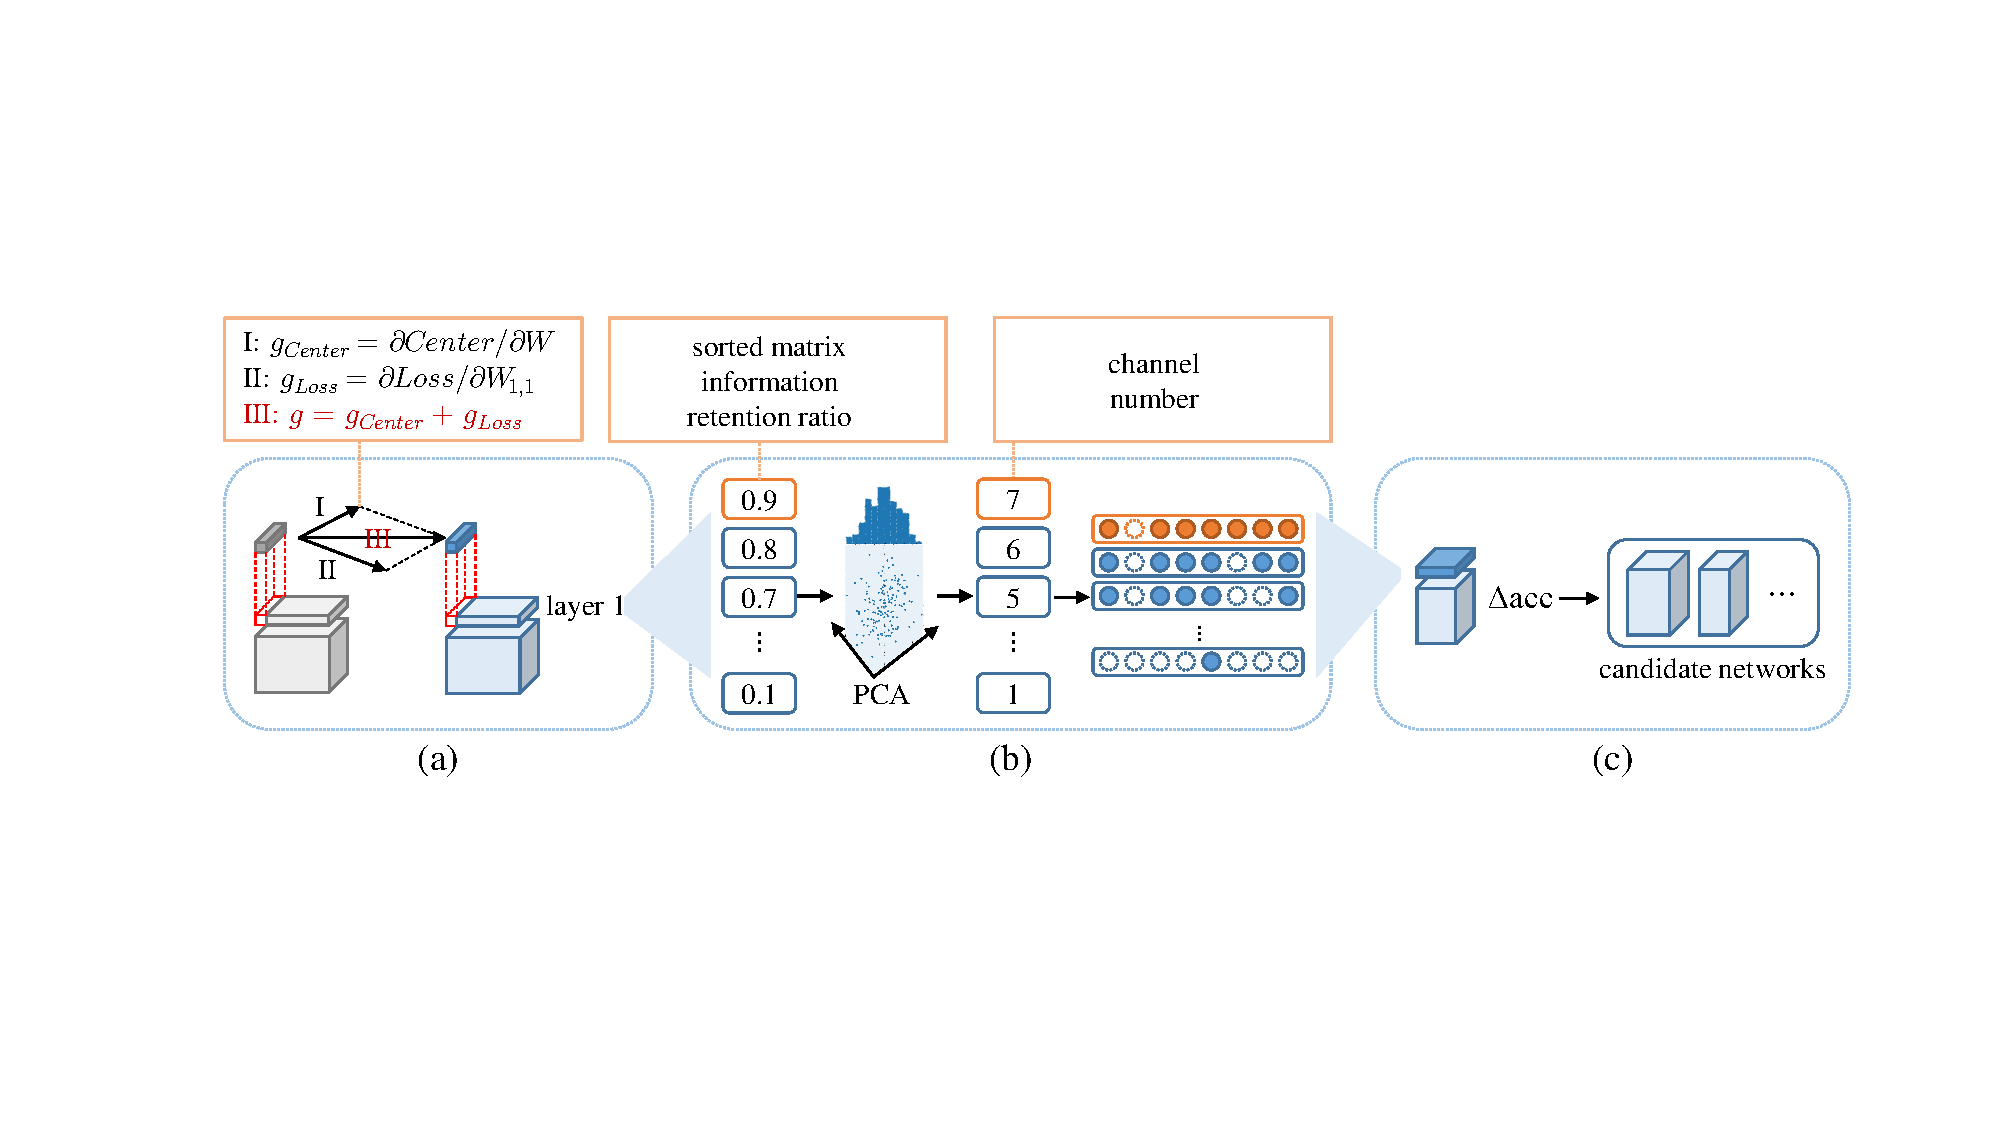
\includegraphics[width=\linewidth]{Fig1.pdf}
   \caption{\textbf{Framework of autoWMC}.  \textbf{(a)} Global centripetal training is applied to the initial network to obtain the to-prune network. \textbf{(b)} Automatic pruning based on the dichotomous search is applied to find the optimal matrix information retention rate, guiding PCA to calculate the channel numbers that can just carry the information of each layer. These numbers will be used as channel clustering targets in cluster-based channel pruning (in the case of layer 1). \textbf{(c)} The pruning result of every exploration will be evaluated, and it will be taken as one of the candidate networks if its loss of accuracy ($\Delta acc$) is acceptable.}
   \label{fig:1}
\end{figure*}

Convolutional Neural Networks (ConvNets) have become increasingly prevalent in a variety of applications, ranging from image classification \cite{2016Deep,2014Very,2016Densely} to detection \cite{2015SSD,2016You,2017Focal,2017Mask} and segmentation \cite{2021INet,2017SegNet,2019Evaluation}. With the advancement of more complex tasks, the size and complexity of ConvNets have expanded significantly \cite{1}. However, this size and computational demand escalation pose substantial challenges for deployment on resource-constrained edge devices like smartphones and tablets \cite{2,2018ShuffleNet}. The intrinsic limitations of these devices in terms of processing power and memory necessitate effective model compression strategies, ensuring that the deployment of sophisticated ConvNets does not compromise their operational efficiency.

Model compression techniques, which include network quantization \cite{3,4,5,6}, knowledge distillation \cite{7}, network pruning \cite{9,10}, network architecture searching (NAS) \cite{11, tan2019efficientnet}. The development of lightweight networks \cite{13,14,15,16} is essential in addressing the dichotomy between the extensive resources required by ConvNets and the limited resources available on edge devices. These techniques aim to maintain an optimal balance between model accuracy and computational cost \cite{17}. In this paper, we focus on channel pruning \cite{lin2021channel,22,24}, a technique that effectively reduces model size while preserving or enhancing its performance. Channel pruning strategically eliminates less important or redundant channels from ConvNets, and fine-tuning ensures minimal loss of accuracy \cite{22,2}. Our study explores this approach's efficacy in deploying complex ConvNet models on resource-limited mobile devices.

In channel pruning for Convolutional Neural Networks, a fundamental approach entails evaluating each substructure within the model to ascertain the most efficient pruning configuration that preserves accuracy. This method, however, faces the challenge of escalating complexity, quantifiable as $O(w^d)$, where $w$ and $d$ represent the network's width and depth, respectively. When coupled with substantial fine-tuning requirements, this complexity often renders the approach impractical for use in resource-constrained environments. Consequently, there is a growing inclination towards search-free pruning methods. One prominent research direction in this domain involves formulating metrics for channel importance to inform the pruning process. While popular, traditional methods in this category, such as batchnorm-based and gradient-based saliency metrics, need a solid theoretical foundation and effectively determine the optimal pruning rate for each layer. An alternative strategy focuses on deriving suitable layer-specific pruning ratios, which typically demands extensive human input and exhaustive sensitivity analysis. This resource-intensive approach poses significant challenges, especially for complex network architectures. Our research addresses these gaps by introducing an innovative channel pruning technique that reduces the reliance on human intervention and balances the dual objectives of maintaining high accuracy and achieving computational efficiency in pruned networks.

\begin{figure*}[t]
  \centering
  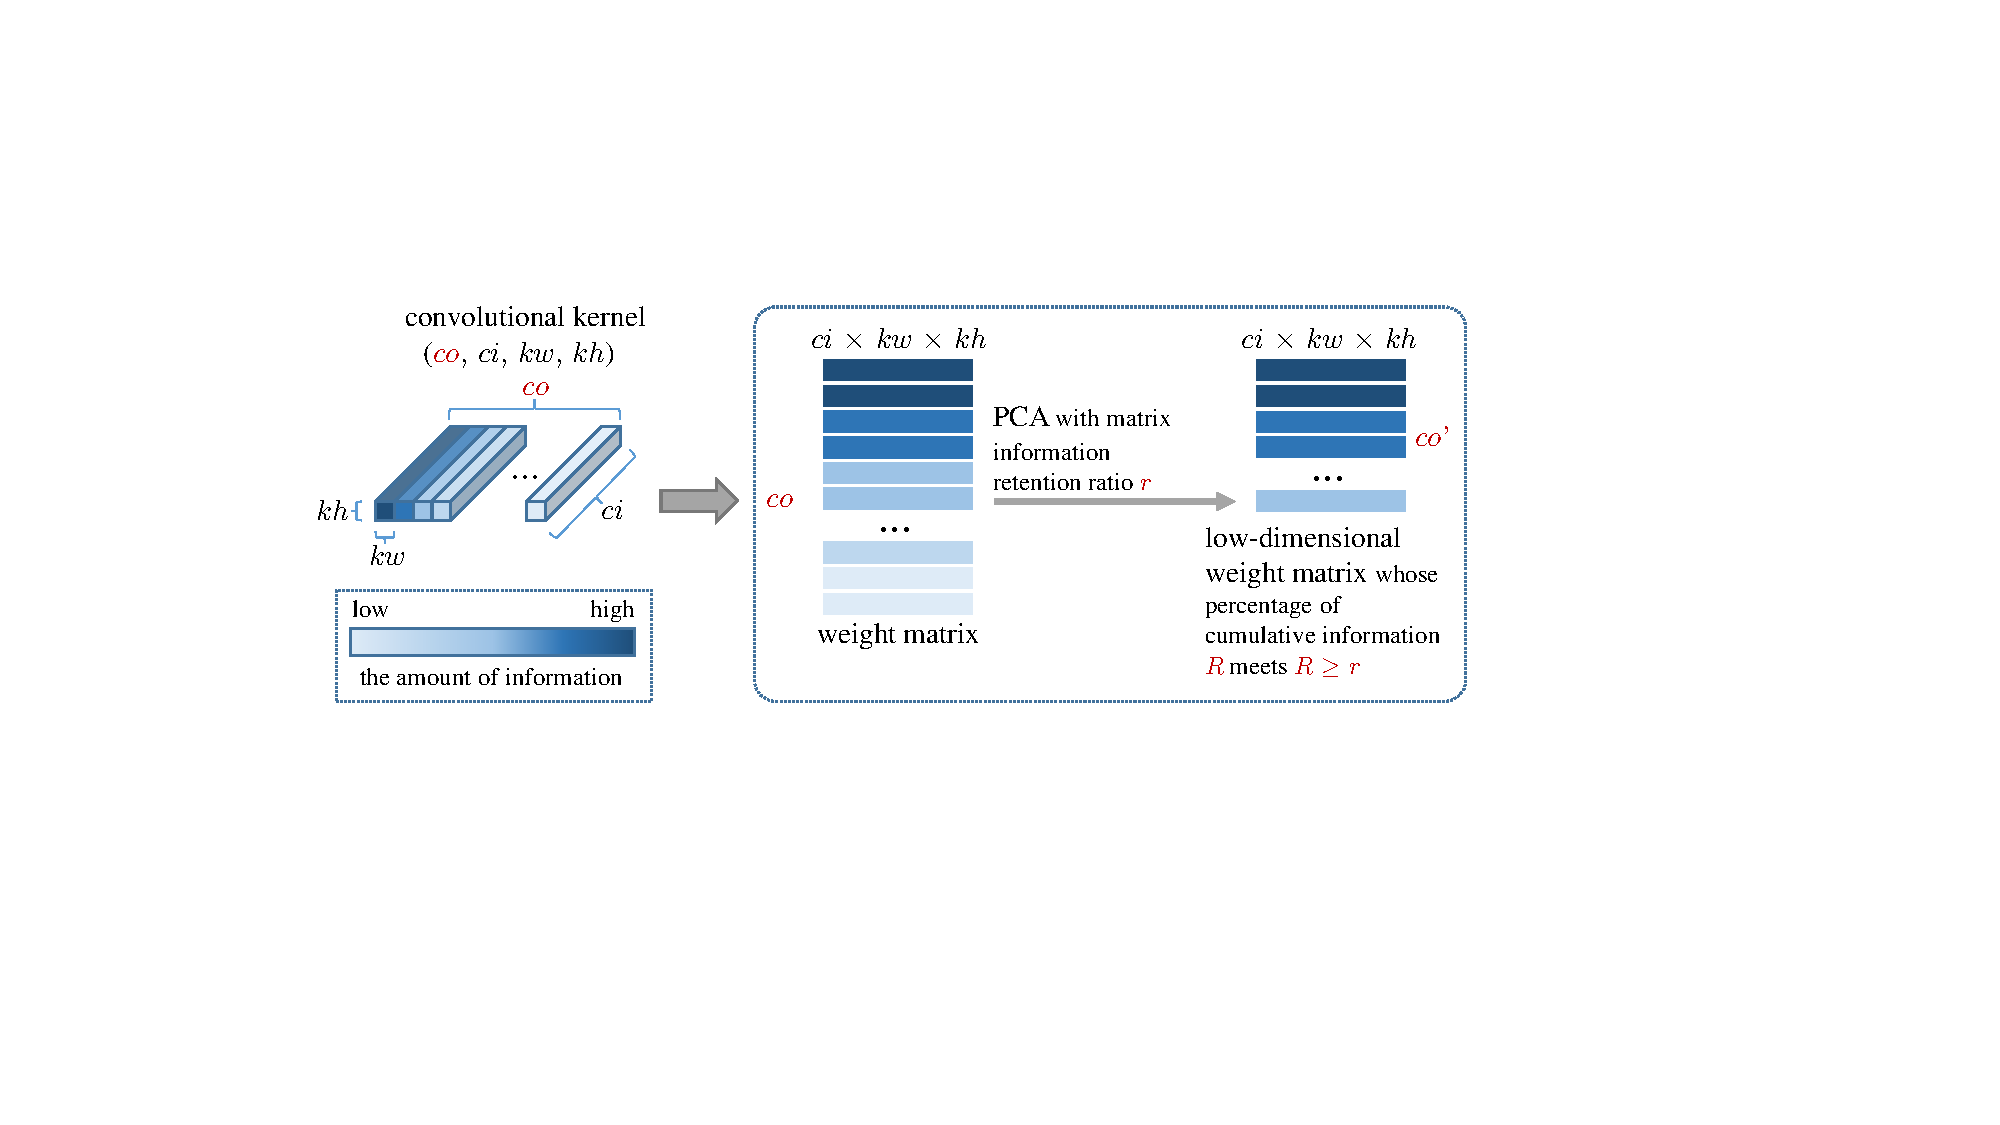
\includegraphics[width=\linewidth]{Fig2.pdf}
   \caption{\textbf{Calculating the channel numbers} based on weight matrix dimensionality reduction, where $co$ denotes the number of original output channels, $co’$ denotes the number of remaining output channels, $ci$ denotes the number of input channels, and $kw$ and $kh$ denote the width and the height of the kernel, respectively. And we represent the amount of information the channel contains by the shade of the cubic color.}
   \label{fig:2}
\end{figure*}

We present autoWMC, an automatic weight matrix con-centration-based channel pruning method, as depicted in Fig. \ref{fig:1}. This method marks a departure from traditional approaches that primarily search for optimal combinations of pruning rates. Instead, autoWMC concentrates on retaining critical information within the weight matrix, utilizing this as a guiding principle for matrix dimensionality reduction. We rank each channel by its contribution to the overall information content of the layer, retaining those channels that contribute most until we achieve the desired information retention ratio. This process is underpinned by linear algebra and information theory principles, enhancing the method's interpretability and ability to adapt the number of channels to each convolutional layer automatically. Our experiments uncovered a challenge associated with neural network over-parameterization, manifested as low similarity between channels and subtle variations in their contributions to the information content \cite{frankle2018lottery,ye2020channel,tzelepis2019deep}. This finding suggests that even minor pruning can significantly impact the network's capacity, thus necessitating extensive fine-tuning to restore accuracy. We have incorporated a concentration concept \cite{35} into our training methodology to counteract this. This approach aims to cluster network parameters more cohesively, enhancing channel similarity and their impact on the information content. The benefit of this is a reduced need for fine-tuning post-pruning. By employing weight matrix dimensionality reduction, autoWMC transforms the traditionally multi-dimensional search for optimal channel numbers across different layers into a more focused search for the most effective information retention ratio within the weight matrix. This substantially narrows down the search space and simplifies the process, requiring just a single user-defined parameter: the tolerable accuracy loss. This allows for the quick generation of a range of candidate-pruned networks. Our extensive experiments across various ConvNet architectures and tasks have demonstrated the universal applicability of autoWMC. Remarkably, autoWMC requires 36\% fewer search epochs than previous methods to achieve similar pruning outcomes with less than 1\% accuracy loss, showcasing its efficiency and effectiveness in model optimization. Our contribution can be summarized as follows:

\begin{itemize}
    \item The information retention ratio we employ offers enhanced interpretability in measuring channel importance, and it automatically adjusts the number of channels in each convolutional layer based on the information content of the layer.
    \item The concentration principle applied in network training promotes channel similarity and diversity in their contributions to information content. Mitigating information loss from pruning effectively reduces the cost of fine-tuning.
    \item The proposed autoWMC allows users to search for the ideal pruned networks in a shorter period by providing only an acceptable loss of accuracy.
\end{itemize}

\section{Related Works}\label{sec2}

Channel pruning, a pivotal technique in model compression, has witnessed various innovative approaches to enhance efficiency while preserving accuracy. The evolution of these methods reflects a deeper understanding of the nuances in neural network architectures.

\textbf{Magnitude-Based Pruning Methods}: This approach initially gained traction due to its simplicity and effectiveness. It operates on the premise that channels with smaller weights contribute less to the network’s output and can be pruned without significant loss of accuracy. The methodology incorporates sparsity-inducing norms, such as the L1-norm, into the loss function. A vital example of this is the work by Li et al., where channel importance is gauged based on the absolute values of weights \cite{18}. This method is straightforward but often overlooks the complex interdependencies between channels, potentially leading to suboptimal pruning decisions.

\textbf{Taylor Expansion-Based Pruning Methods}: To address the limitations of magnitude-based approaches, newer methods based on Taylor expansion have been developed. These methods challenge the assumption that smaller weights are less informative. Molchanov et al.'s approach is a notable example, where pruning decisions are made through a fine-tuned balance of removing channels and preserving network performance \cite{20}. This method iteratively evaluates the impact of channel removal, using Taylor expansion to estimate the change in the loss function, thus allowing for a more nuanced pruning strategy.

\begin{figure*}[t]
  \centering
  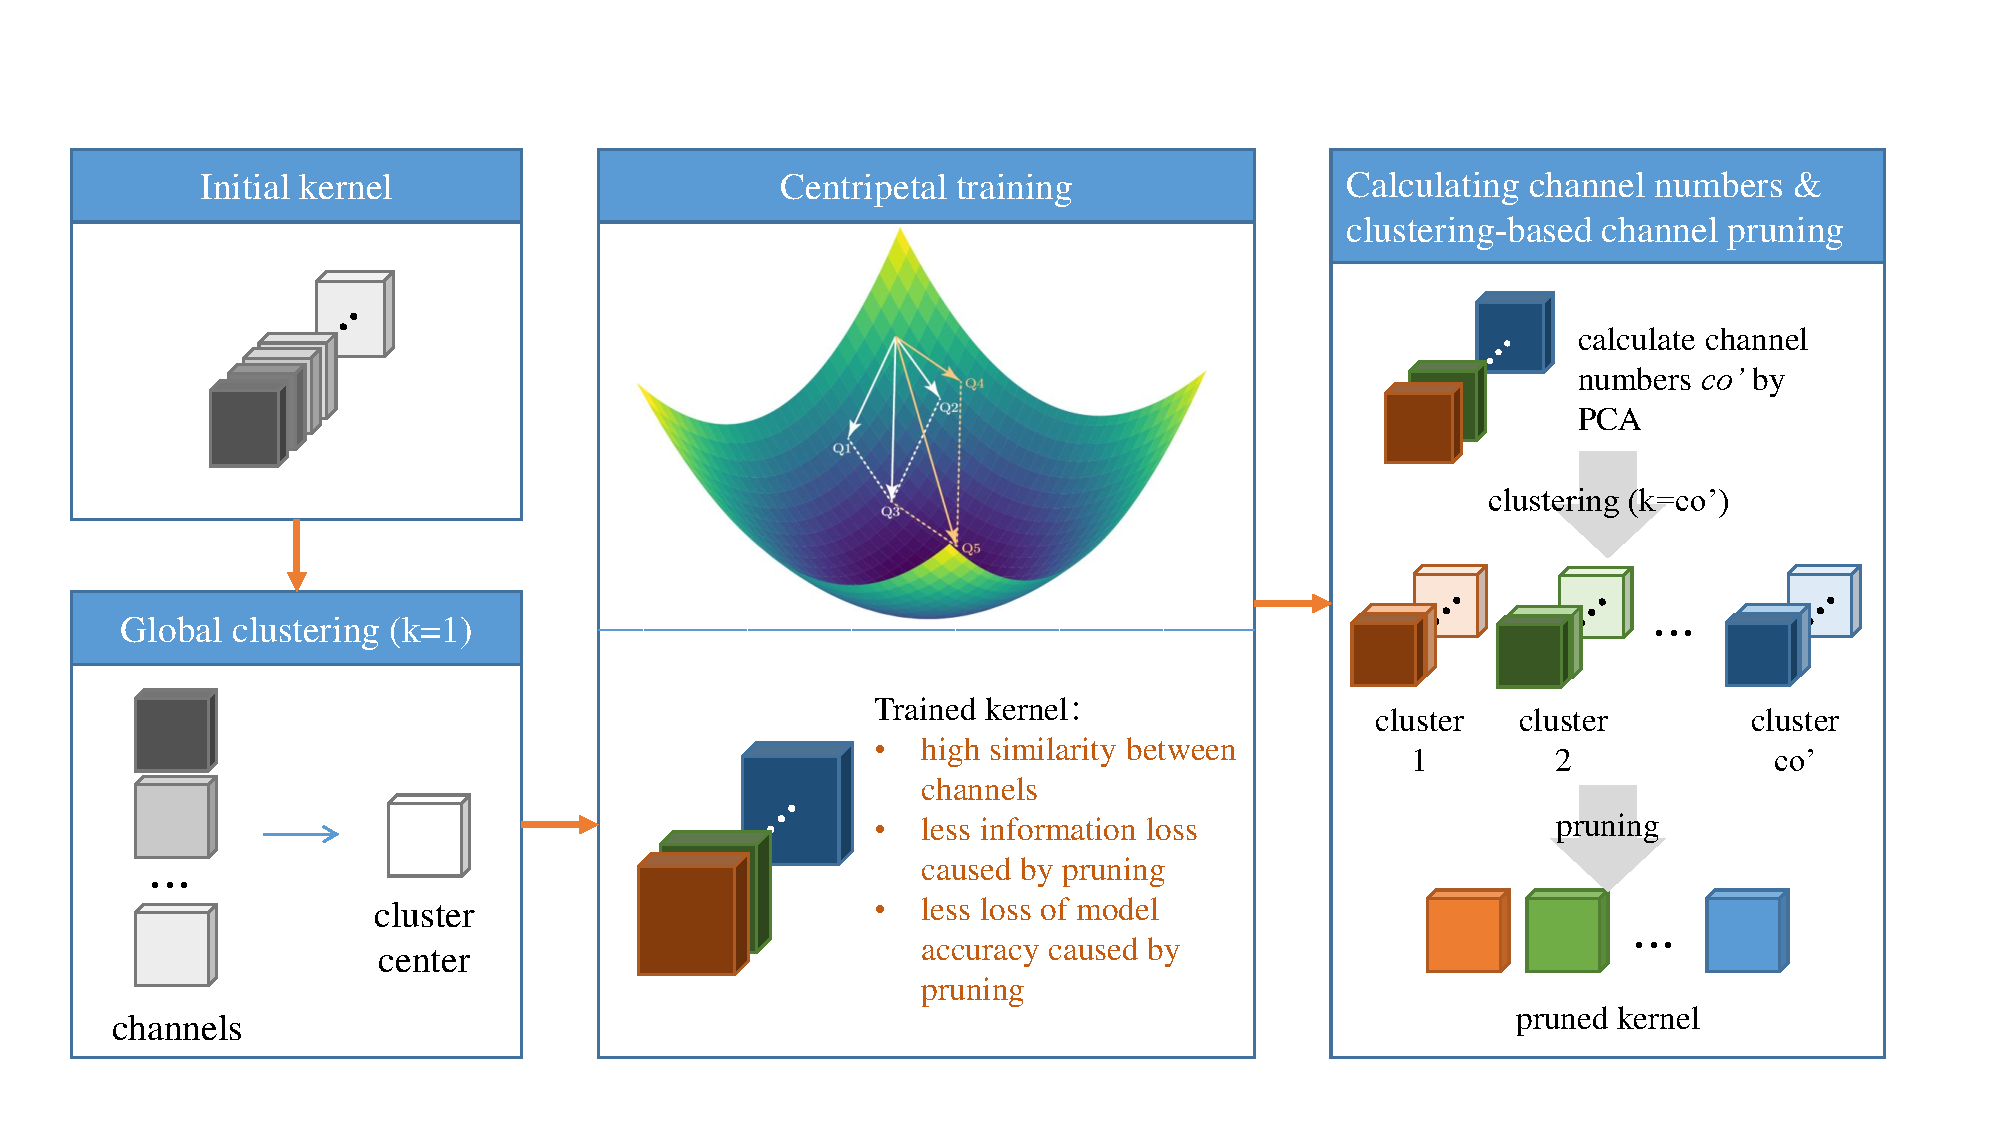
\includegraphics[width=\linewidth]{Fig3.pdf}
   \caption{\textbf{The clustering-based channel pruning with global centripetal training}. The initial kernel is globally clustered ($k=1$) to obtain a cluster center, and the channels of the kernel would get closer to it while fitting the targets during centripetal training. Furthermore, the channel number $\textit{co'}$ is calculated for each layer by PCA which is used as the target of channel clustering.}
   \label{fig:3}
\end{figure*}

\textbf{Reconstruction-Based Pruning Methods}: These methods represent a shift towards understanding the functional impact of channels on network output. Luo et al. and He et al. pioneered this approach, focusing on the feature output of convolutional layers. By assessing the similarity of feature outputs between the pruned and original models, channels deemed least significant to output reconstruction are pruned \cite{21,22}. This method is particularly effective in identifying channels whose removal has minimal impact on the overall network performance, thereby maintaining accuracy post-pruning.

In recent developments, the focus has shifted towards understanding the intricate relationships between network weights and their collective impact on model performance. This shift is evident in methods that employ more holistic and systemic approaches:


\textbf{Reinforcement Learning-Based Methods}: Ashok et al. utilized reinforcement learning to identify optimal strategies for layer removal and shrinkage \cite{23}. This method is part of a broader trend of employing advanced machine learning techniques to optimize network structures, representing a significant departure from more traditional, heuristic-based approaches.

\textbf{Quadratic Programming and Clustering Methods}: Recent studies by Peng et al. and Zhuo et al. have approached channel pruning from a mathematical optimization and clustering perspective, respectively \cite{24,tzelepis2019deep}. These methods offer a more systematic approach to pruning, considering the network architecture as a whole rather than individual channels in isolation.

The setting of the pruning ratio remains a critical aspect of channel pruning. Traditional methods often rely on a predefined global pruning ratio, which may only be optimal for some layers. This realization has led to the development of more sophisticated approaches that determine layer-specific pruning ratios, as highlighted in the studies by Han et al. and Li et al. \cite{18,2015Learning}. These methods are based on the understanding that different layers have varying sensitivities to pruning, necessitating a more tailored approach.

In contrast to predefined methods, the latest research is increasingly gravitating towards automatic pruning techniques. These techniques dynamically calculate the pruning ratio during the training process, adapting to the unique characteristics of each network layer. For instance, Liu et al. applied L1 regularization to Batch Normalization layers to induce sparsity \cite{29}, while Singh et al. and Idelbayev et al. developed frameworks that alternate between training and pruning phases to gradually converge to an optimal network structure \cite{30,31}.

Our work with autoWMC represents a significant advancement in this field. Building upon the foundations laid by previous research, autoWMC introduces a novel approach that focuses on the pruned network's overall structure and weight inheritance. By requiring only a threshold for acceptable accuracy loss, autoWMC simplifies determining the optimal pruning strategy. This method stands out for its ability to automatically identify the most effective pruning ratio, thereby reducing the reliance on extensive manual analysis and experimentation. Our experiments demonstrate that autoWMC is versatile and practical across various ConvNet architectures and tasks, marking a significant step forward in model compression.


\section{Methodology}\label{sec3}

In the realm of network pruning, our focus lies on a to-prune network \( M \) characterized by \( L \) convolutional kernels (layers), each with a specific channel configuration denoted by \( C = \{c_1, c_2, \ldots, c_L\} \). Here, \( c_i \) represents the number of channels in the \( i \)-th kernel. The objective of clustering-based channel pruning is to eliminate redundant channels—those that are similar or identical—thereby deriving an optimally pruned structure \( M^* \) with a revised channel configuration \( C^* = \{{c_1}^*, {c_2}^*, \ldots, {c_L}^*\} \), where \( 1 \le {c_i}^* \le c_i \) for each layer.

This pruning approach analyzes each convolutional kernel \( K_i \) in the original network \( M \). It involves categorizing the channels into \( {c_i}^* \) clusters and preserving only one representative channel from each cluster. This process effectively reduces redundancy within each kernel \( K_i \), contributing to constructing the pruned network \( M^* \), which retains the most distinctive and informative channels from the original structure.

However, pursuing the optimal pruned structure \( M^* \) presents a significant computational challenge. The most straightforward strategy would be to exhaustively explore every possible substructure \( M' \) with varying channel combinations \( C' = \{c_1', c_2', \ldots, c_L'\} \), where \( 1 \le c_i' \le c_i \). The sheer number of potential substructures for a network with \( L \) layers is given by the product of the channel counts across all layers, mathematically represented as \( \prod_{i=1}^{L}c_i \) \cite{lin2021channel}. Such an exhaustive search demands an impractical number of computational probes, rendering this approach infeasible for networks of substantial complexity.

To address this challenge, our proposed method, AutoWMC, introduces a more efficient approach to determining the optimal channel combination \( C' \). Rather than embarking on an exhaustive search, AutoWMC calculates \( C' = \{c_1', c_2', \ldots, c_L'\} \) based on the quantity of information contained within each kernel. This calculated channel combination is then applied to the clustering-based channel pruning process. By prioritizing the retention of information-rich channels, AutoWMC significantly reduces the computational burden of finding the optimal pruned network structure, thus offering a more viable and efficient solution to channel pruning in convolutional neural networks.

\subsection{Calculation of the channel numbers}

\begin{figure}
  \centering
  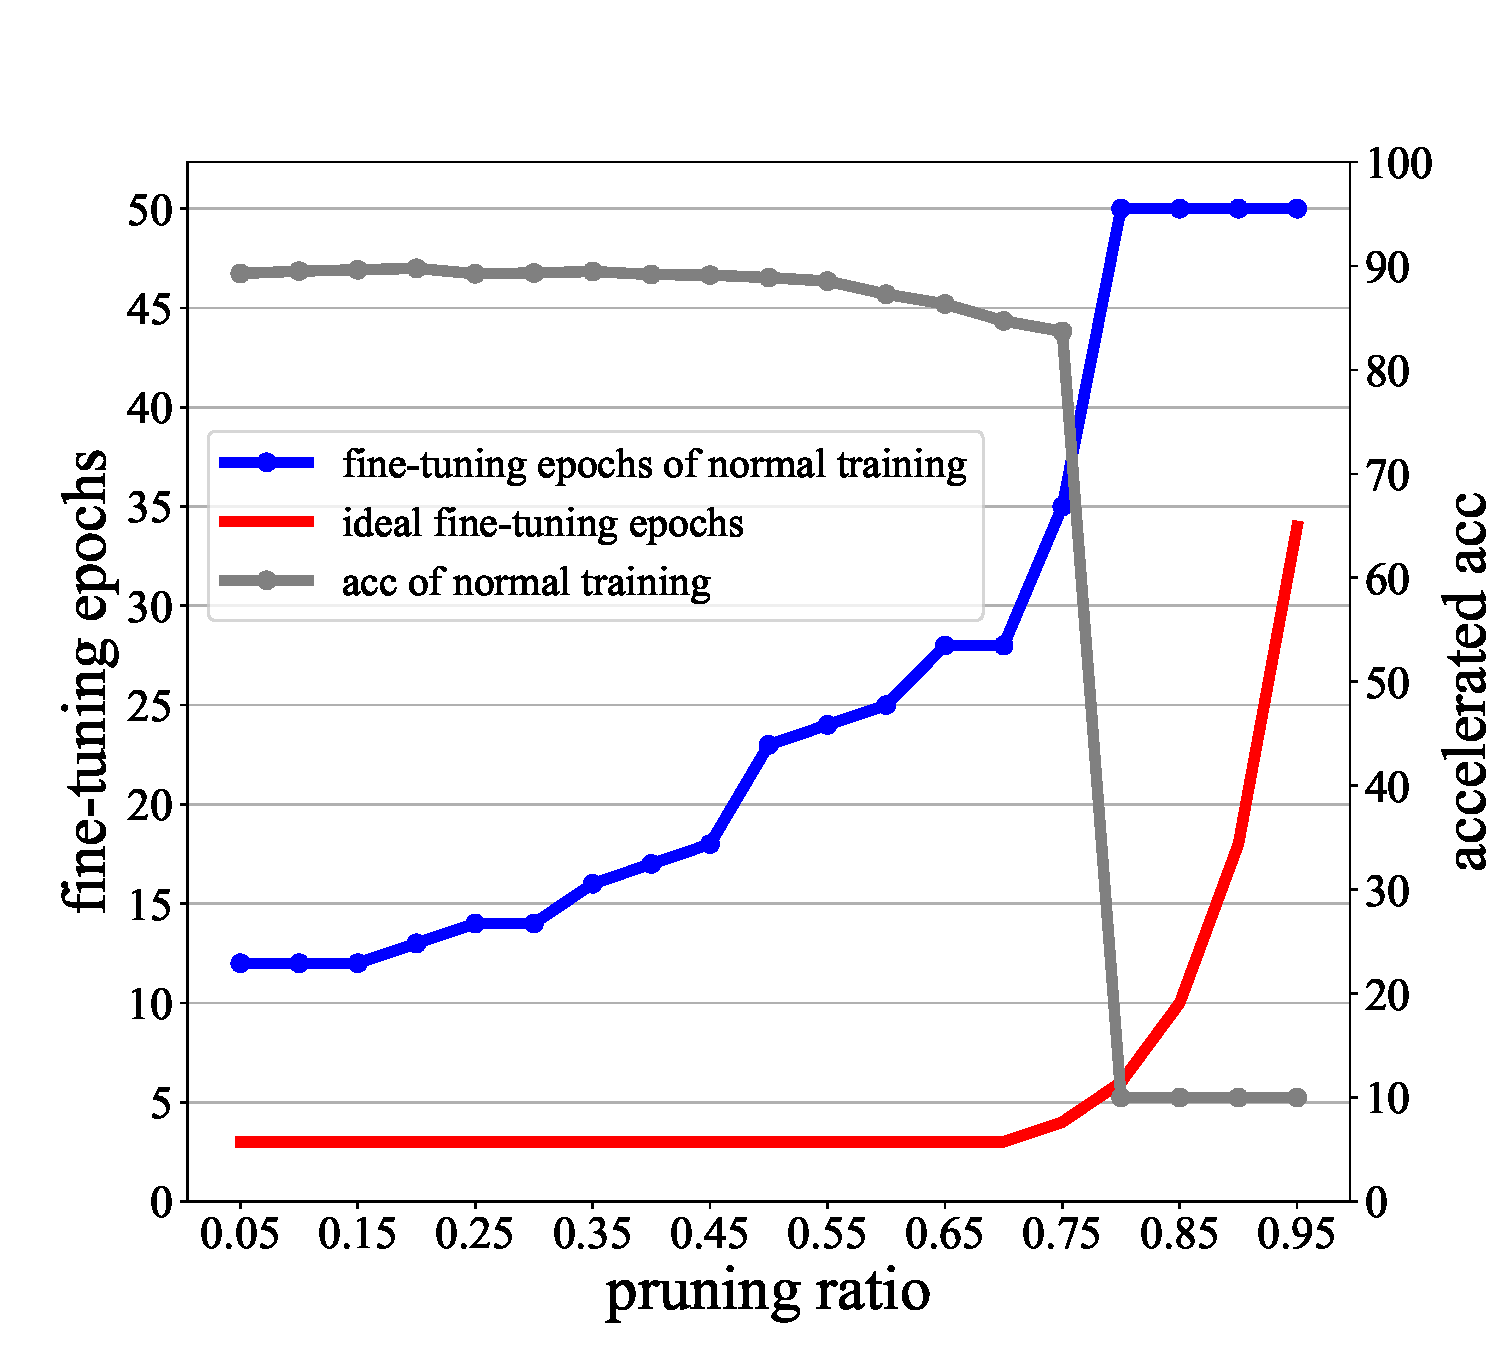
\includegraphics[width=\linewidth]{Fig4.pdf}
   \caption{\textbf{The curve of pruning ratio, fine-tuning epochs, and accuracy of ResNet50 on CIFAR10}, where the blue and red lines denote the required fine-tuning epochs and ideal fine-tuning epochs at different pruning ratios, respectively, and the grey line denotes the accelerated accuracy.}
   \label{fig:4}
\end{figure}

Low-rank decomposition, a channel pruning method grounded in linear algebra, offers a novel approach to determining the optimal number of channels for convolutional kernels. By transforming a convolutional kernel \( K \) into a weight matrix \( W_K \) and seeking a lower-dimensionality matrix to replace it, this method prunes redundant channels effectively \cite{2020Low}. The crux of this technique lies in expanding \( W_K \) using a maximal linearly independent group \( {W_K}^* \), where the information content of \( {W_K}^* \) is equivalent to the information entropy of \( W_K \). Consequently, the rank \( r_{W_K} \) of \( W_K \), which is the dimensionality of \( {W_K}^* \), is identified as the optimal channel number \( {c_k}^* \) for \( K \), sufficient for conveying the requisite information. However, the challenge emerges when dealing with fully trained networks, whose weight matrices are typically full-rank, leaving no prune channels. As a solution, matrix dimensionality reduction is adopted, aiming to reduce the number of channels while striving to retain as much information as possible. This balance ensures that low-rank decomposition remains an effective tool for channel pruning, particularly when information preservation is crucial.


\begin{figure*}[t]
  \centering
  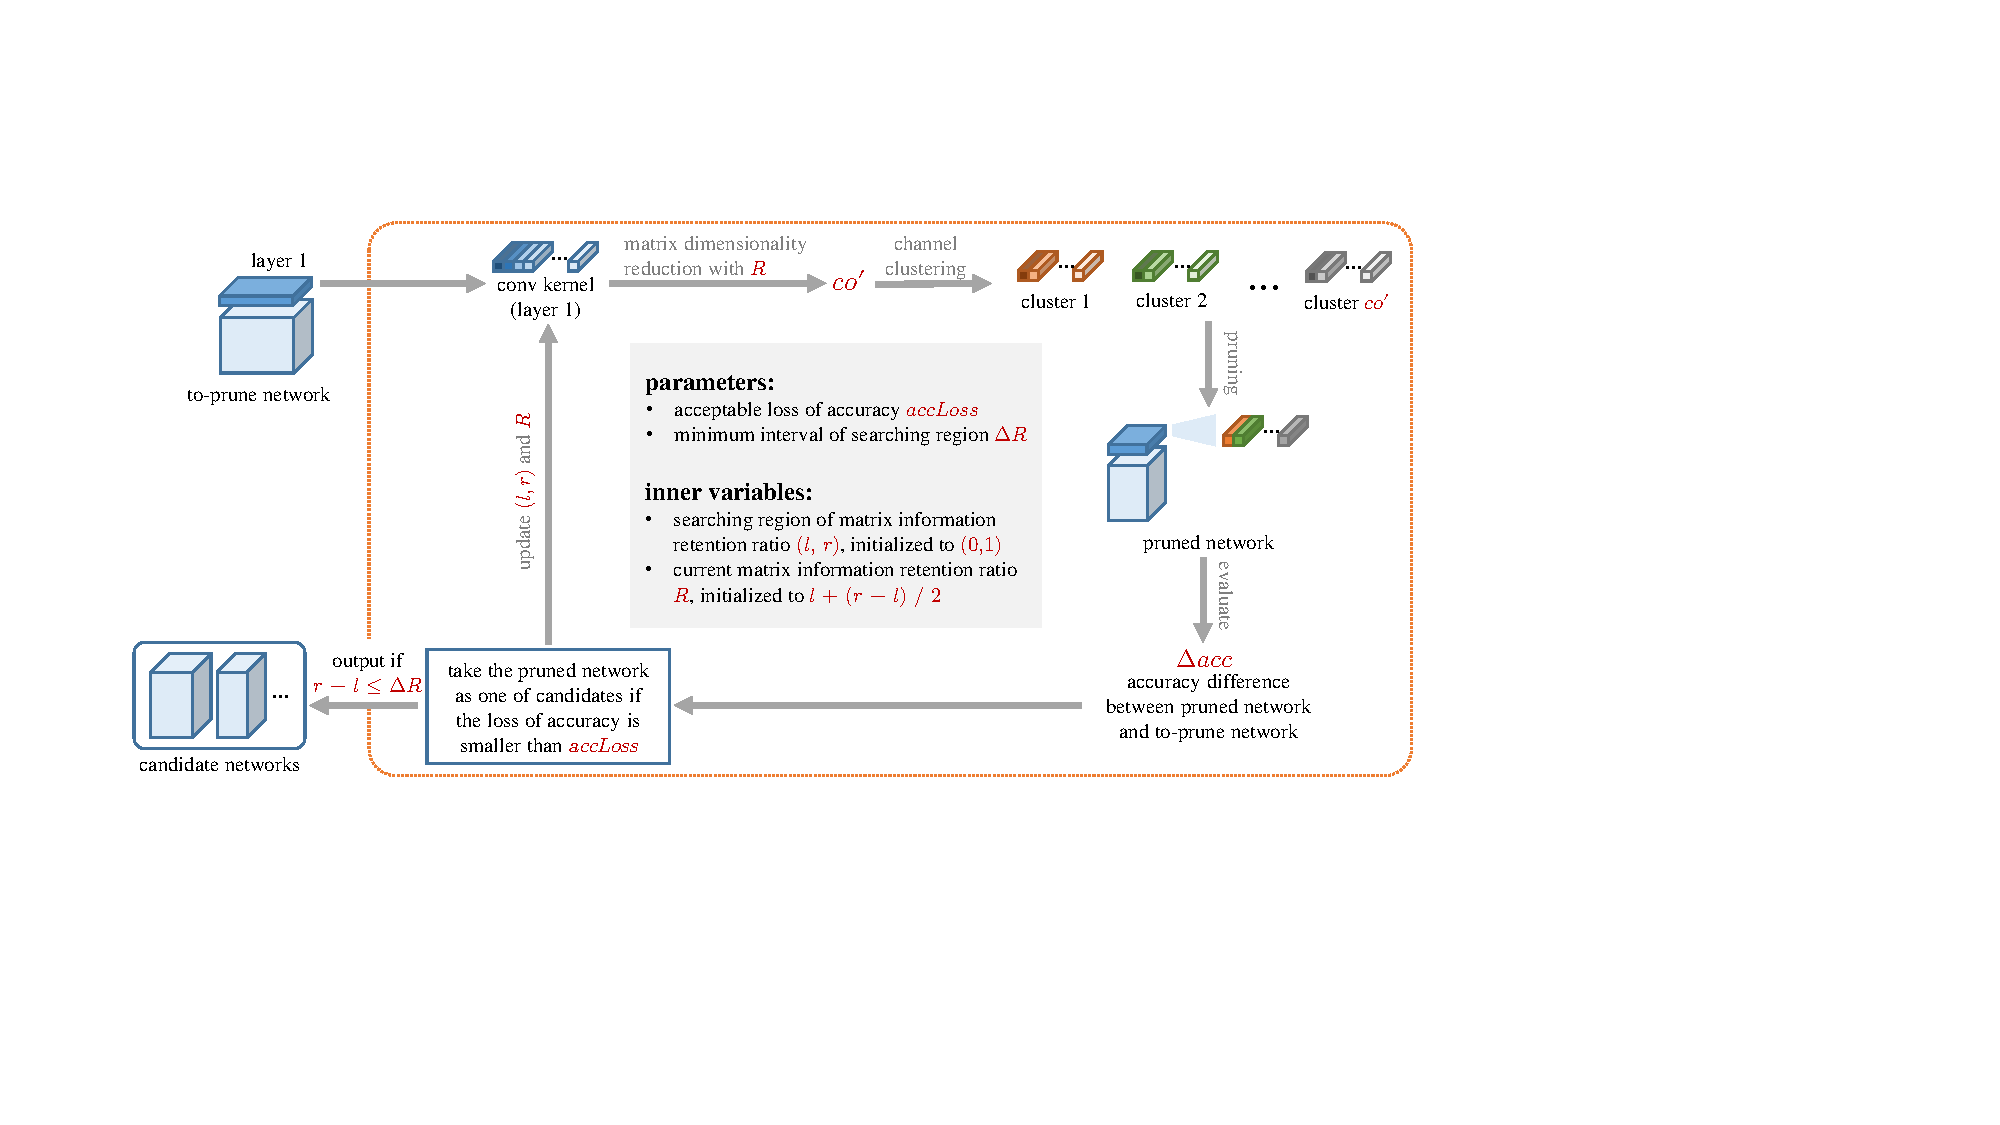
\includegraphics[width=\linewidth]{Fig5.pdf}
   \caption{\textbf{Automatic pruning based on dichotomous search}, where $co'$ denotes the channel number calculated by PCA, and $\Delta acc$ is the metric to decide if a pruned network will be taken. The algorithm has two parameters: 1) $accLoss$, which denotes the acceptable accuracy loss of the pruned networks, and 2) $\Delta R$, which denotes the minimum searching region where the algorithm ends when the current searching region is smaller than it. Moreover, the algorithm has three inner variables, the current explored matrix information retention ratio $R$ and the boundaries of the current searching region $(l,r)$. Layer 1 is an example to show the searching process for the matrix information retention ratio.}
   \label{fig:5}
\end{figure*}


Principle Component Analysis (PCA), a well-established technique in matrix dimensionality reduction, plays a pivotal role in calculating the optimal channel numbers for convolutional kernels, as illustrated in Figure \ref{fig:2}. PCA operates by eigendecomposing the covariance matrix, \({\rm mat}_{cov}\), derived from the weight matrix \( W \) of a redundant kernel. This process yields a set of eigenvalues, each representing the variance contribution of the corresponding vectors in \( W \), as delineated in Equation \ref{eq:1}. Here, \(\mathrm{\Lambda}\) is the diagonal matrix where each diagonal element quantifies the variance contribution, effectively indicating the amount of information each vector carries.

\begin{equation}
    {\rm mat}_{cov}=\frac{W^TW}{n-1}=Q\mathrm{\Lambda}Q^T,
    \label{eq:1}
\end{equation}

The channel selection is guided by the hyper-parameter \( r \) (where \( 0 < r < 1 \)), known as the cumulative variance contribution rate. Channels with higher variance contributions are retained until the cumulative rate meets or exceeds \( r \), as defined in Equation \ref{eq:2}. Applying this criterion across all kernels results in a new channel combination \( C' \), optimally balancing information retention and dimensionality reduction.


\begin{equation}
    \frac{\sum_{remained\ vectors}\varepsilon_i}{\sum_{all\ vectors}\varepsilon_i}\geq r,
    \label{eq:2}
\end{equation}

This PCA-based approach significantly simplifies the channel pruning problem. The complexity of exploring potential channel combinations, previously \( O(n^L) \), is now reduced to determining the appropriate range for \( r \), simplifying the complexity to \( O(n) \). This reduction not only streamlines the channel pruning process but also ensures that the most informative channels are preserved, enhancing the efficiency and efficacy of the model compression.

\subsection{Global centripetal training}

Fine-tuning is an indispensable process in restoring the accuracy of a neural network following channel pruning, primarily due to the resultant diminution in network capacity. This reduction often necessitates a recalibration of the pruned model to achieve the original level of accuracy. As depicted in Figure \ref{fig:4}, a discernible trend is observed where the number of fine-tuning epochs required increases proportionately to the pruning ratio. The blue line in the figure graphically represents this. Ideally, our objective is to minimize the number of fine-tuning epochs needed at any given pruning ratio, as illustrated by the red line in the figure, thereby effectively curtailing the associated computational costs.

The rationale behind the increased need for fine-tuning is that channel pruning, even at modest ratios, can significantly deplete the information content within the network's kernels. This depletion is attributed to the original uniform distribution of learned target information across all the network channels. To counteract this loss of information, we have innovated a novel approach named 'centripetal training,' predicated upon the concept of global clustering. This technique, elucidated in Figure \ref{fig:3}, encompasses the amalgamation of all channels into a singular cluster. This is followed by a strategic realignment of these channels towards a collective center during subsequent training phases. The mechanics of this process are further detailed in Equation \ref{eq:3} \cite{35}.

\begin{equation}
\begin{aligned}
    F^{(j)} &\leftarrow F^{(j)}+\tau \Delta F^{(j)},
    \\ 
    \Delta F^{(j)} &= -\frac{\sum_{k \in H(j)} \frac{\partial L o s S}{\partial F^{(k)}}}{|H(j)|}-\eta F^{(j)}+\epsilon K,
    \\
    K &= \frac{\sum_{k \in H(j)} F^{(k)}}{|H(j)|}-F^{(j)},
    \label{eq:3}
\end{aligned}
\end{equation}

The cornerstone of our centripetal training approach is a meticulously crafted weight update rule designed to augment the similarity among the channels. This similarity is pivotal in mitigating the adverse effects typically associated with channel pruning, particularly concerning the network's capacity. In the context of each kernel's \( j \)-th channel, this methodology involves the precise calculation of both the weights \( F^{(j)} \) and their respective updates \( \Delta F^{(j)} \). The update process itself is dependent on the channel cluster \( H(j) \), which includes the \( j \)-th channel. A synergy of several factors orchestrates this process: the learning rate \( \tau \), the objective function \( Loss \), the weight decay factor \( \eta \), and a critical hyper-parameter \( \epsilon \) – designated as the centripetal strength. The value of \( \epsilon \) is paramount, as it governs the extent of centripetalization, effectively consolidating the channel weights towards a unified cluster center.

This method facilitates a more concentrated distribution of target information throughout the network and enhances channel congruence. Consequently, the fine-tuning cost is substantially reduced, courtesy of minimizing the pruning-induced detriment to the network's capacity. This efficiency translates into reduced fine-tuning epochs necessary to recuperate the accuracy lost due to pruning. The empirical results from our experiments substantiate these claims, indicating a significant reduction in the number of fine-tuning epochs required while concurrently maintaining or augmenting the network's accuracy.


\subsection{Automatic pruning framework}

Acknowledging the intricate relationship between pruning ratio and accuracy, as illustrated by the orange line in Figure \ref{fig:4}, we adopt a dichotomous search strategy in our autoWMC methodology for effective channel pruning, as shown in Figure \ref{fig:5}. This strategy revolves around optimizing the matrix information retention ratio, a crucial internal variable guiding the pruning process. Our approach begins with a given network \( M \), for which the channel combination \( C' \) is computed using PCA under the guidance of the current matrix information retention ratio \( R \). This computation intricately balances the need to reduce the network's complexity while preserving its essential information content.

In the subsequent step, for each convolutional kernel in the network, denoted as the \( i \)-th kernel, the channels are grouped into \( c_i' \) clusters. Only a single representative channel is retained from each cluster to form the pruned network \( M' \). This selective retention ensures that the most critical features of the network are preserved. The viability of \( M' \) as a candidate network is determined based on whether the resultant accuracy loss falls within an acceptable threshold. If deemed viable, \( M' \) is added to a set of potential solutions, and the internal variables are accordingly adjusted for further refinement of the search.

The process iterates, narrowing down the search range of the matrix information retention ratio until it reaches a pre-established minimal interval. This iterative refinement is crucial in identifying the optimal candidate network set that balances efficiency and accuracy. The culmination of this process yields a set of optimally pruned networks, each striking a balance between minimal structural complexity and maximal performance retention.

The autoWMC algorithm streamlines the pruning process by treating the matrix information retention ratio as an adjustable internal variable. This treatment significantly simplifies the pruning task, requiring only two parameters to initiate: an acceptable loss of accuracy (\( accLoss \)) and a minimum interval for the search region (\( minInterval \)), in addition to the initial network configuration. The algorithmic steps of this process are systematically outlined in Algorithm \ref{alg:AOA}. This algorithm demonstrates the efficiency and effectiveness of autoWMC, providing a robust framework for navigating the complex landscape of network pruning. By integrating a thoughtful balance between computational resource expenditure and model accuracy, autoWMC represents a significant advancement in the field of neural network optimization.



\begin{algorithm}[!h]
    \caption{autoWMC.}
    \label{alg:AOA}
    \renewcommand{\algorithmicrequire}{\textbf{Input:}}
    \renewcommand{\algorithmicensure}{\textbf{Output:}}
    \begin{algorithmic}[1]
        \REQUIRE initial network: $initNet$, acceptable loss of accuracy: $accLoss$, minimum interval of searching region: $minInterval$.
        \ENSURE the set of candidate networks: $candidateSet$.

        \STATE  generate $M$ by applying global centripetal training to $initNet$

        \STATE  $l \leftarrow 0.0$, $r \leftarrow 1.0$

        \STATE  obtain $originalAcc$ by evaluating $M$
        \WHILE{$l + minInterval \leq r$}
            \STATE $R \leftarrow l + (r – l) / 2$
            \STATE generate $C^\prime$ by PCA under the guidance of $R$
            \STATE generate $M^\prime$ by pruning $M$ according to $C^\prime$
            \STATE obtain $acc$ by evaluating $M^\prime$
            \IF {$acc + accLoss \leq originalAcc$}
                \STATE candidateSet.append($M^\prime$)
                \STATE $r \leftarrow R$
            \ELSE
                \STATE $l \leftarrow R$
            \ENDIF
        \ENDWHILE
        
        \RETURN $candidateSet$
    \end{algorithmic}
\end{algorithm}

\section{Experiments}

\subsection{Results of calculating channel numbers}

To evaluate the effectiveness of PCA in calculating channel numbers, we conducted experiments on the VGG16 and ResNet34 models, provided by \textit{torchvision} and pre-trained on ImageNet. We set a range of matrix information retention ratios \(
\varepsilon \in \{ 0.2, 0.4, 0.6, 0.8, 0.9, 0.95, 1 \}
\) to investigate their impact on the channel calculation.

The results, as depicted in Figure \ref{fig:6}, reveal notable variations in calculated channel numbers across different kernels, even within the same model. For instance, in VGG16 (Figure \ref{fig:6a}), the channel numbers between kernels like \textit{features.17} and \textit{features.28} differ under the same \(\varepsilon\). Similarly, in ResNet34 (Figure \ref{fig:6b}), kernels such as \textit{layer.3.0.conv1} and \textit{layer.3.5.conv2} also display varying channel numbers. This variation underscores the inherent differences in information content across different kernels, validating the rationale behind adjusting channel numbers to reflect the unique informational characteristics of each kernel under a uniform matrix information retention ratio.

\begin{figure}
  \centering
  \begin{subfigure}{1\linewidth}
  \centering
    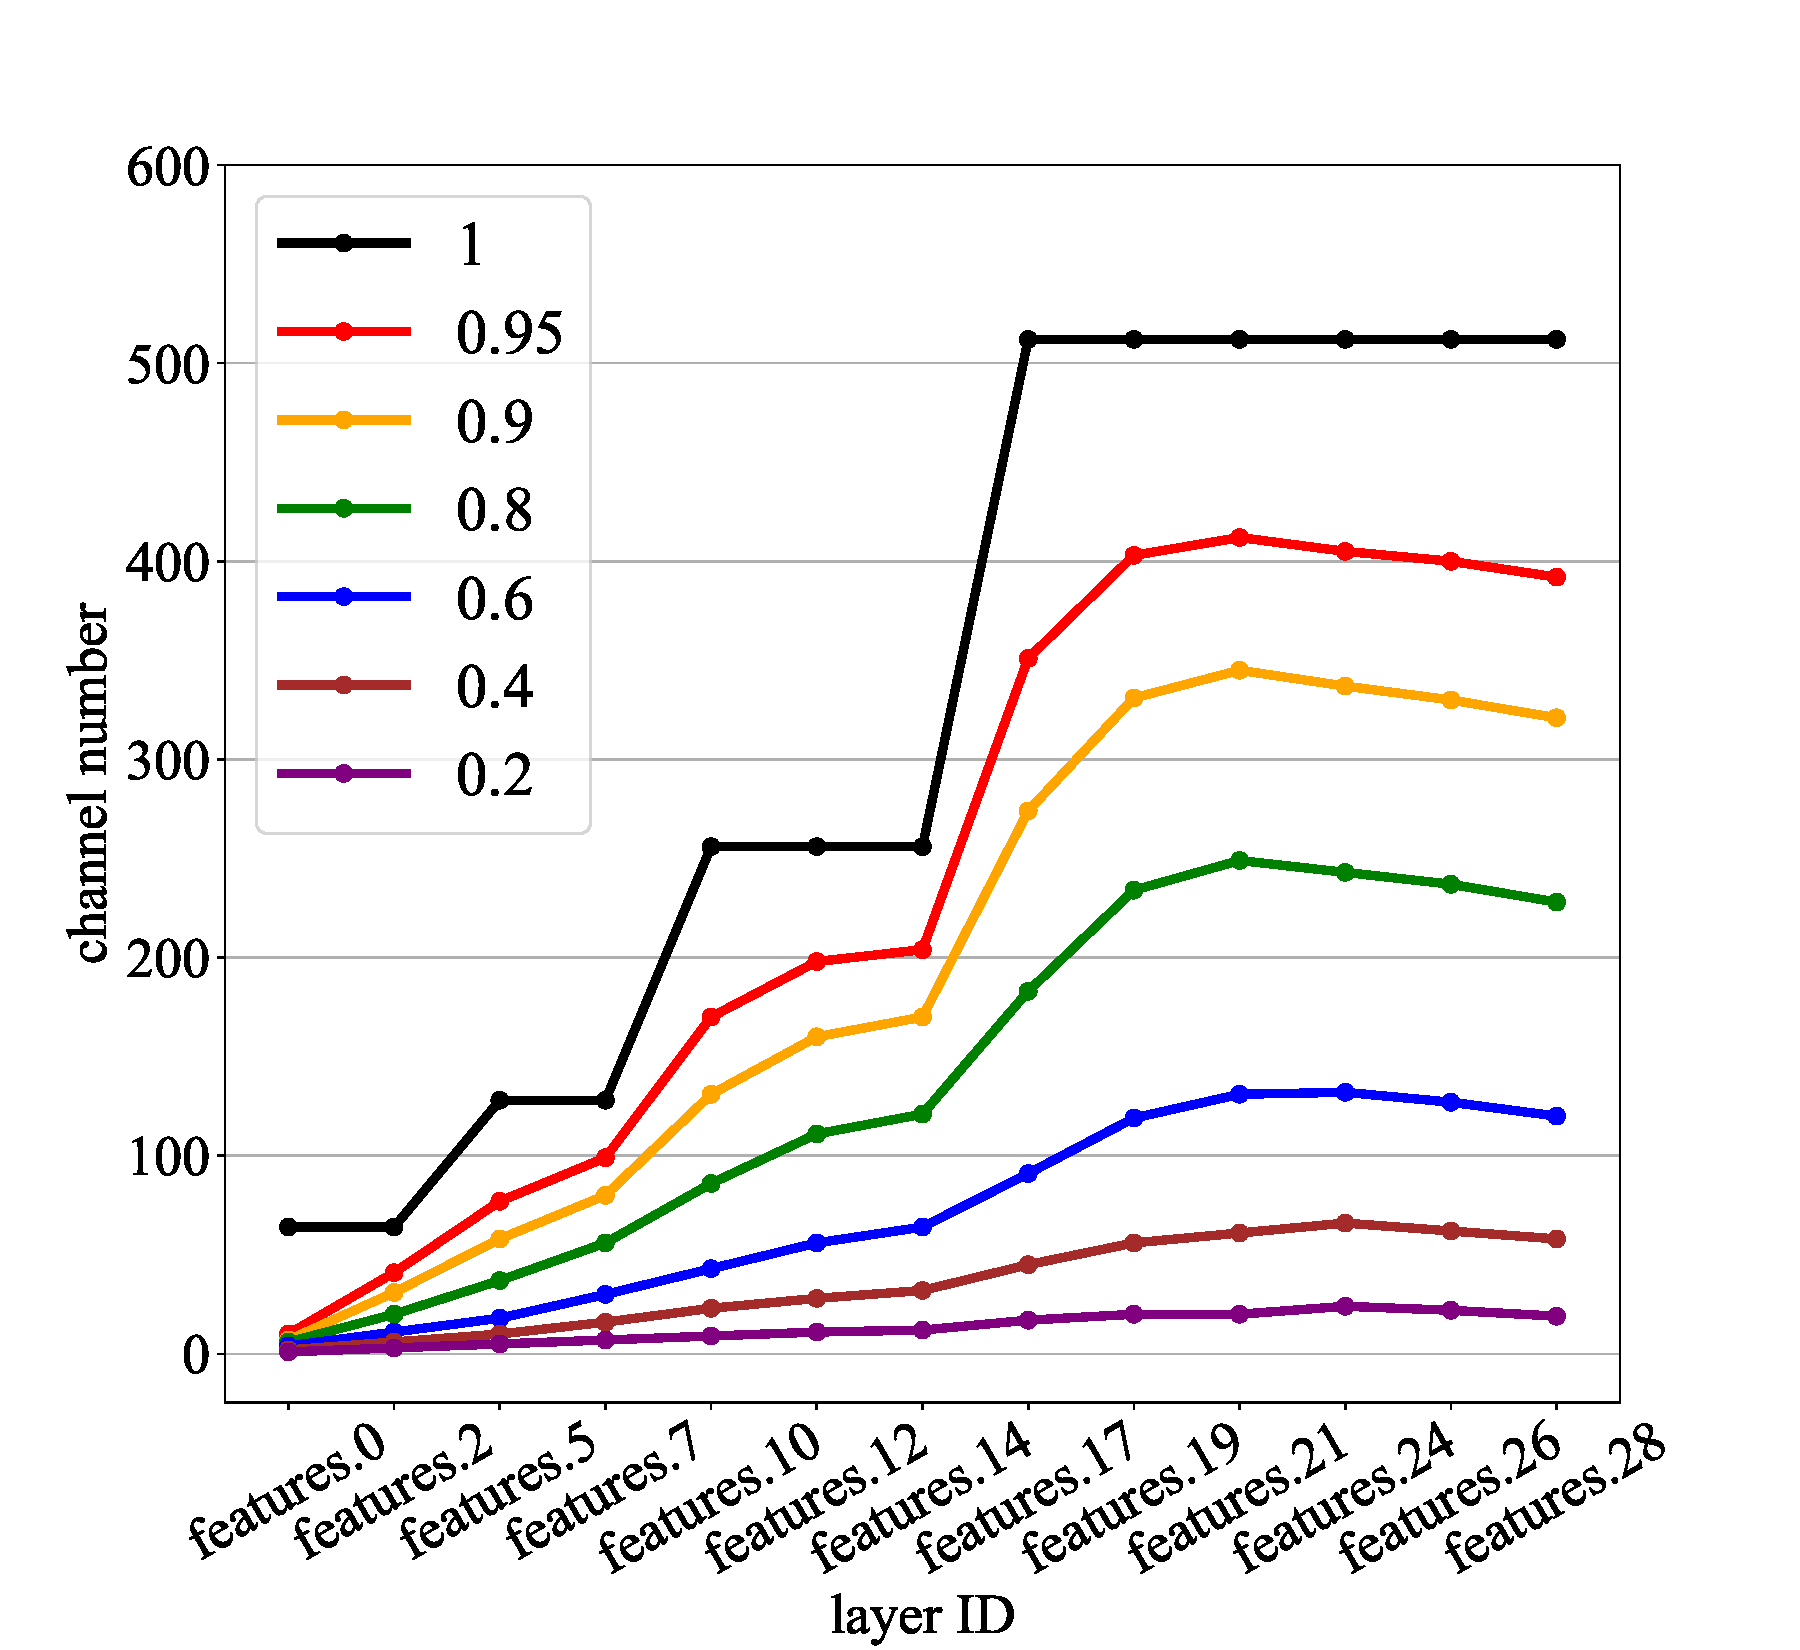
\includegraphics[width=\linewidth]{Fig6a.pdf}
    \caption{}
    \label{fig:6a}
  \end{subfigure}
  \vspace{0.2pt}
  \begin{subfigure}{1\linewidth}
  \centering
    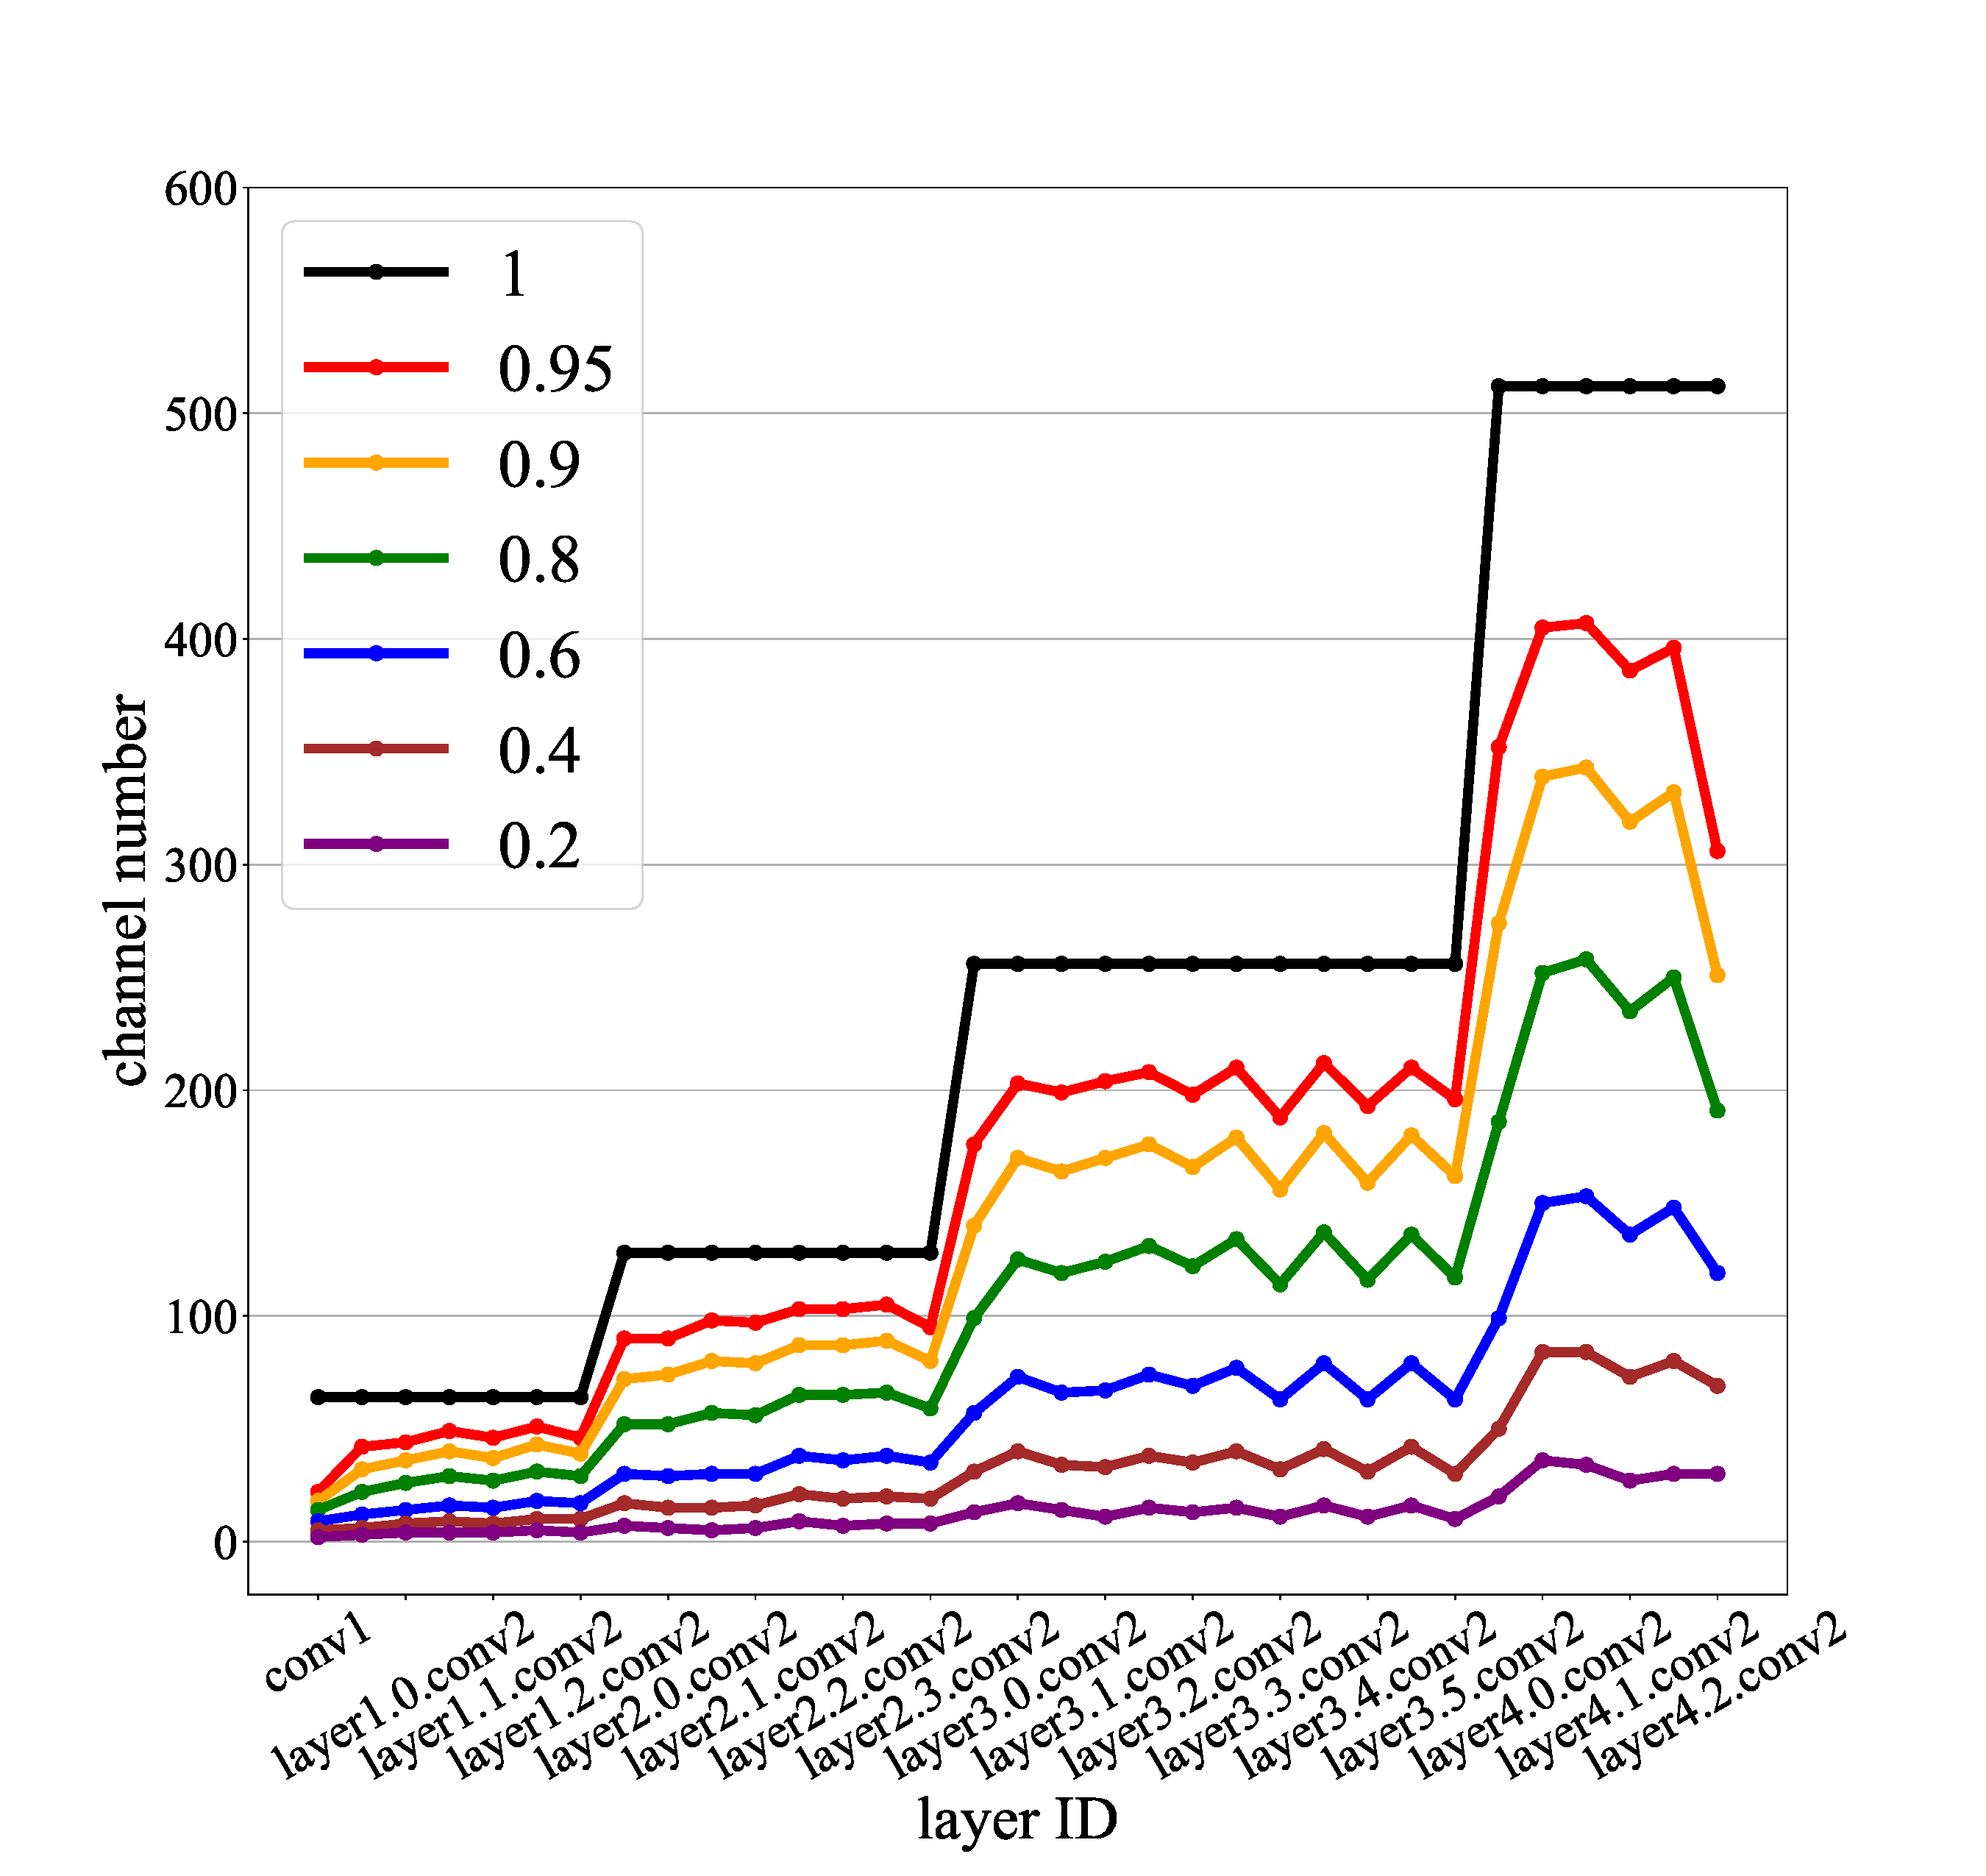
\includegraphics[width=\linewidth]{fig6b.pdf}
    \caption{}
    \label{fig:6b}
  \end{subfigure}
  \caption{\textbf{The channel numbers calculated based on PCA for different kernels of VGG16 \textbf{(a)} and ResNet34 \textbf{(b).} This figure shows how channel numbers vary under different matrix information retention ratios, represented by various colored curves. Each color signifies a different ratio, detailing the impact on pruning across kernels. The curve for a retention ratio of 1 highlights the original channel numbers, serving as a baseline for understanding PCA's pruning effect on network architecture.}}
  \label{fig:6}
\end{figure}


\begin{figure}
  \centering
  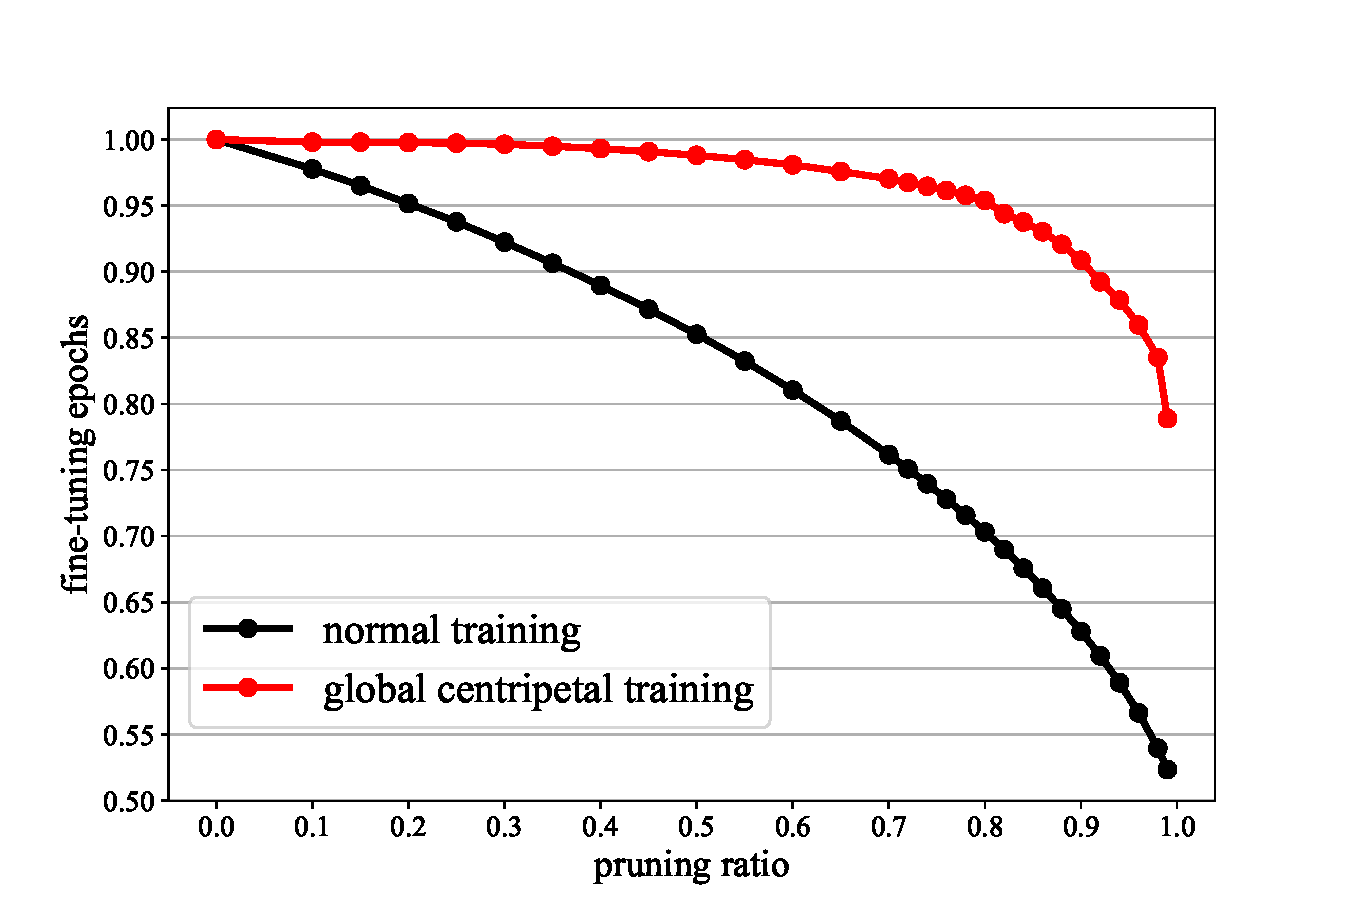
\includegraphics[width=\linewidth]{Fig7.pdf}
   \caption{\textbf{The information retention ratio curves of ResNet50 with different pruning ratios on CIFAR10}, where the black line denotes the curve of information retention ratios of a regularly trained ResNet50 at different pruning ratios, which declines steadily, and the red line denotes the curve of the ResNet50 of global centripetal training which has a lower rate of information loss.}
   \label{fig:7}
\end{figure}


\begin{figure}
  \centering
   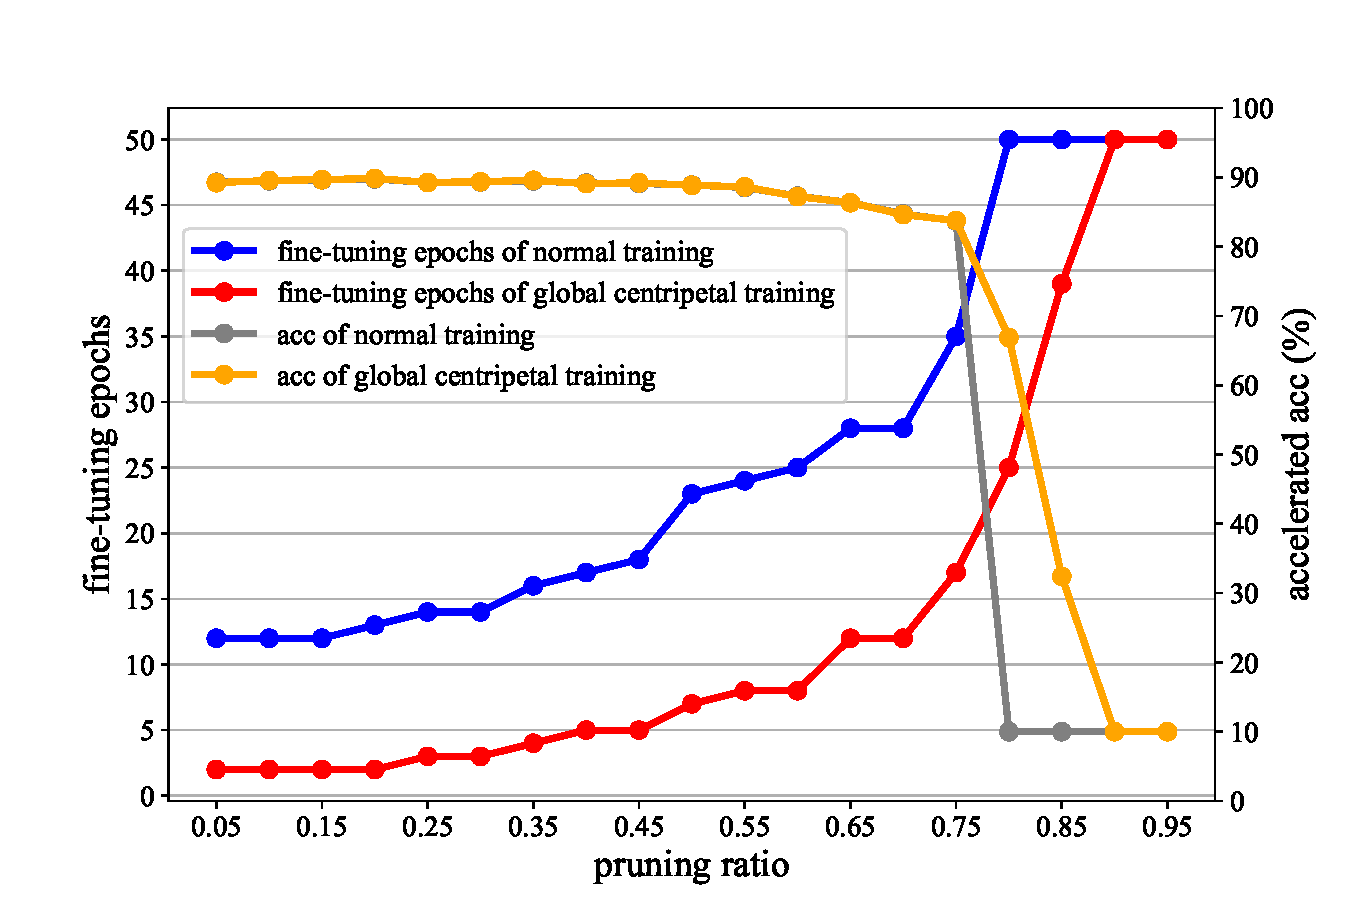
\includegraphics[width=\linewidth]{Fig8.pdf}
   \caption{\textbf{The epochs of the fine-tuning and accuracy curves of ResNet50 with different pruning ratios on CIFAR10}, where the blue and orange lines denote the required fine-tuning epochs of the ResNet50 of regular training and global centripetal training, respectively. The red line is more similar to the red line shown in Figure \ref{fig:4}. The grey line and the yellow line denote accelerated accuracy, respectively.}
   \label{fig:8}
\end{figure}

Moreover, despite these variations, the general trends across different retention ratios (represented by different colors in Figure \ref{fig:6}) remain consistent. This consistency aligns with the theoretical understanding that the proportional change in channel numbers under different \(\varepsilon\) values should be relatively uniform, given a fixed amount of information in the kernels. Hence, the similarity in trends across different curves corroborates our methodological approach and provides valuable insights into the dynamic relationship between information retention and channel distribution in convolutional neural networks.


\subsection{Results of global centripetal training}

To rigorously validate the effectiveness of global centripetal training, we conducted a comprehensive experiment using the ResNet50 model, specifically trained on the CIFAR10 dataset. Our experimental design involved a detailed training regimen spanning 300 epochs, employing Stochastic Gradient Descent (SGD) as the optimization technique. Crucially, global centripetal training was introduced in the 101st epoch. The rationale behind this phased approach was grounded in the initial condition of the network weights. At the outset, these weights are randomly initialized, implying that any early application of global clustering (\(k=1\)) would be tangential to task-specific learning, possibly undermining the accuracy of the final model. By initially abstaining from centripetal training for the first 100 epochs, we allowed the network to adapt and align itself more closely with the target task, ensuring that the channel cluster centers formed in the later stages of training were more relevant and conducive to the task at hand.

The impact of this training strategy is vividly captured in Figure \ref{fig:7}, which delineates the information retention ratio curves for the ResNet50 model under various pruning ratios. In the case of the network that underwent regular training, a stable and gradual decrease in information retention is observed as the pruning ratio is incremented (illustrated by the black line). This trend contrasts markedly with the behavior of the network trained with global centripetalization. Here, we notice a more pronounced and steep decline in the information retention ratio (depicted by the orange line). This steeper curve indicates a more concentrated distribution of target information within the network and a higher degree of redundancy among the pruned channels. Such a pattern unequivocally demonstrates that global centripetal training effectively amplifies the focus on crucial information, thereby mitigating the detrimental effects typically associated with the pruning process.

Further insights are gleaned by examining the fine-tuning epochs required for the network under different pruning ratios, as shown in Figure \ref{fig:8}. This comparative analysis reveals that applying global centripetal training substantially reduces the number of fine-tuning epochs needed to regain the pre-pruning level of accuracy. The reduction in fine-tuning effort corroborates the enhanced efficacy of global centripetal training and resonates with our overarching goal of curtailing fine-tuning costs. It underscores the method's proficiency in preserving network performance post-pruning while significantly diminishing the extent of additional training required. This outcome is a testament to the strategic advantage of incorporating global centripetal training in the network pruning process, highlighting its role in streamlining model optimization and maintenance.



\subsection{Results of autoWMC}

In this section, we evaluate the efficacy of autoWMC using four performance metrics: 1) FLOPs, representing the number of floating-point operations; 2) Params, indicating the total number of network parameters; 3) Acc, denoting the accuracy achieved on the test set; and 4) searching cost (in epochs), quantifying the computational effort required for automatic pruning.

Two experiments were conducted to validate autoWMC's capabilities:

1) autoWMC was applied to various networks trained on CIFAR10 for 300 epochs using SGD, with global centripetal training initiated at the 101st epoch. We set the acceptable accuracy loss at 1\% and the minimum interval of the searching region at 0.01. Table \ref{tab1} shows a significant reduction in FLOPs and Params, particularly in networks like ResNet50, which demonstrated a compression rate exceeding 95\%. This high reduction rate is attributable to the surplus capacity of ResNet50 for the CIFAR10 dataset, underscoring autoWMC's ability to tailor network complexity to specific tasks effectively.

2) Two instances of a pre-trained ResNet50 from \textit{torchvision} were trained on ILSVRC-2012 for 160 epochs, with one undergoing global centripetal training starting from the 51st epoch. Maintaining the same criteria for acceptable accuracy loss and searching region interval as the first experiment, we observed from Table \ref{tab2} that autoWMC, particularly when combined with centripetalization, outperformed state-of-the-art methods by 0.18\% in accuracy, while also reducing the searching cost by nearly 30\%. Compared to methods like ABCPruner\cite{lin2021channel}, autoWMC achieved comparable pruning results but with the added advantage of simplifying the pruning process. Unlike methods that rely on technical experience for setting hyperparameters, autoWMC requires only an acceptable accuracy loss to commence, making it more user-friendly, especially for non-expert users.

These experiments demonstrate that autoWMC achieves competitive or superior pruning results and significantly reduces the computational cost and complexity involved in the pruning process, making it an effective tool for optimizing neural networks in various settings.


\begin{table}[]
\centering
\begin{tabular}{lccc}
\hline
Model & FLOPs ↓\% & Params ↓\% & Acc \\ \hline
VGG16 & 78.19 & 56.28 & 88.12(-0.96) \\
ResNet50 & 95.07 & 95.70 & 87.57(-0.97) \\
ResNet34 & 86.35 & 91.20 & 89.38(-0.72) \\
AlexNet & 46.86 & 27.80 & 84.99(-0.76) \\
DenseNet121 & 92.70 & 93.56 & 86.88(-0.26) \\
GoogLeNet & 66.19 & 49.85 & 90.21(-0.85) \\ \hline
\end{tabular}
\caption{\textbf{Automatic pruning results of different networks on CIFAR10}. The output of autoWMC is a collection of pruning results with acceptable accuracy loss compared with the to-prune network. The data in the table shows the pruned network with the highest compression rate among the candidates.}
\label{tab1}
\end{table}

\begin{table}[]
\centering
\begin{tabular}{lccc}
\hline
Method & FLOPs $\downarrow$\% & Acc & Cost \\ \hline
Baseline & - & 76.01 & - \\
ThiNet-50\cite{21} & 58.7 & 71.01 & 244 \\
metaPruning\cite{liu2019metapruning} & 29.5 & 74.49 & 160 \\
ABCPruner\cite{lin2021channel} & 38.2 & 74.84 & 102 \\
Ours (accLoss=.01, w/o. C) & 36.7 & 75.10 & 137 \\
Ours (accLoss=.01, w. C) & 35.5 & 75.02 & \textbf{98} \\ \hline
\end{tabular}
\caption{\textbf{Searching cost (epochs) of different pruning frameworks for ResNet50 on ILSVRC-2012}, where w/o. C and w. C denote without global centripetal training and with global centripetal training, respectively.}
\label{tab2}
\end{table}


\section{Limitation}

In our clustering-based channel pruning method, the randomness of preserving one channel per cluster can lead to varying outcomes in different experiments, even under the same configuration. This issue impacts the reproducibility and consistency of results. Additionally, the dichotomous search in automatic pruning is susceptible to decision bias when accuracy loss nears the acceptable threshold. To address these challenges, adopting deterministic criteria for channel selection and refining the decision-making mechanism in the dichotomous search could help stabilize the process and enhance the consistency and reliability of the pruning outcomes.


\section{Conclusion}

We have presented an automatic channel pruning method centered around the concentration of convolutional layer weight matrices. By employing matrix dimensionality reduction, we tailor the channel numbers for each convolutional layer, effectively managing the complexity of more profound and broader ConvNets. The key to our approach is using the matrix information retention ratio as the hyperparameter, stabilizing the search space for channel combinations regardless of network scale. To further optimize the pruning process, we introduce global centripetal training. This technique enhances channel similarity, significantly reducing the fine-tuning cost by mitigating the information loss typically associated with pruning. Additionally, using dichotomous search in the automatic pruning process efficiently compresses the search space for the optimal network substructure. This method only requires an acceptable loss in accuracy to swiftly identify the most effective pruning results, offering a user-friendly approach to network optimization. Our approach represents a significant advancement in automatic channel pruning, promising reduced computational overhead and enhanced effectiveness.

%%
%% The next two lines define the bibliography style to be used, and
%% the bibliography file.
\bibliographystyle{ACM-Reference-Format}
\bibliography{sample-base}



\end{document}
\endinput
%%
%% End of file `sample-authordraft.tex'.
